\documentclass[10pt, conference, compsocconf]{IEEEtran}

\usepackage{graphicx}
\usepackage{amsmath}
\usepackage{hyperref}
\usepackage[utf8]{inputenc}
\usepackage[T1]{fontenc}
%\usepackage{float}
\usepackage{listings}
\usepackage{color}
%\usepackage{amssymb}
\usepackage{ifsym}
%\usepackage{algorithm}
%\usepackage{algorithm2e}
%\usepackage{algpseudocode}
%\usepackage[ruled,vlined,linesnumbered]{algorithm2e}
%\usepackage[]{algorithm2e} 

\usepackage[english]{babel}
\usepackage[utf8]{inputenc}
\usepackage{algorithm}
\usepackage[noend]{algpseudocode}
\usepackage{amssymb}


\definecolor{dkgreen}{rgb}{0,0.6,0}
\definecolor{gray}{rgb}{0.5,0.5,0.5}
\definecolor{mauve}{rgb}{0.58,0,0.82}

\lstset{frame=tb,
  language=C++,
  aboveskip=3mm,
  belowskip=3mm,
  showstringspaces=false,
  columns=flexible,
  basicstyle={\small\ttfamily},
  numbers=none,
  numberstyle=\tiny\color{gray},
  keywordstyle=\color{blue},
  commentstyle=\color{dkgreen},
  stringstyle=\color{mauve},
  breaklines=true,
  breakatwhitespace=true,
  tabsize=3
}
\title{Subspace clustering on objects with constraints}
\author {Vamshi Bhushanaboina \\  {vamshi.bhushanaboina@st.ovgu.de} 
   \and Majed Ali  \\ {majed.ali@ovgu.de} 
   \and Nikhil Raikar \\ {nikhil.raikar@st.ovgu.de}}
% *** CITATION PACKAGES ***
%
\ifCLASSOPTIONcompsoc
  % The IEEE Computer Society needs nocompress option
  % requires cite.sty v4.0 or later (November 2003)
  \usepackage[nocompress]{cite}
\else
  % normal IEEE
  \usepackage{cite}
\fi


% *** GRAPHICS RELATED PACKAGES ***
%
\ifCLASSINFOpdf	

\else

\fi


\begin{document}
\maketitle
\markboth{}%
{{Name1, Name2}: (title)}
\IEEEtitleabstractindextext


\begin{abstract}
For any clinical decisions to be made, the set of associated features leading to those decisions play a major role. The discovery of those associated features are based on set of labeled examples and also the analysis of fundamental information of the features with  respect to the target variable. however this may not be the case since obtaining large sets of labeled examples may not be feasible, In these cases instead of considering the value of the target variable, expert knowledge on similarity has been taken and has been derived in 
DRESS(Discovery of relevant example-constrained subspaces) algorithm[1] having them yielding good results. In our approach we take the same relevant algorithm and use a different clustering process. we propose a adaptive semi-supervised clustering approach based on multiple density-based information which can automatically determine sets of important densities in use of both labeled and unlabeled data. Based on these parameters we identify complex structures in different sizes and shapes without any prior information of the number of clusters.This approach has been generally evaluated on SHIP-2 Dataset and has yielded promising clustering results.

\textit{Keywords-}medical data mining, patient similarity, feature selection,
classification, epidemiological studies, hepatic steatosis
%Hash-based aggregation strategy is used for performing grouped aggregation queries.
%However, this strategy has high processing time for result computation. In this work,
%we explore the use of code optimization strategies to reduce the execution time. we
%introduce a way to perform insertion along with probing in the underlying hashing
%techniques. We also exploit the SIMD capability of modern hardwares to speed up
%the hashing technique operations. In our work, we evaluate the performance of scalar
%and vectorized execution of hashing-based aggregation with cuckoo hashing and linear
%probing as underlying hashing techniques. We use different dataset distributions for our
%evaluation. We also evaluate the impact of group size on runtime for computing grouped
%aggregation. Finally, we provide our inferences on the evaluation results obtained.
\end{abstract}
\IEEEdisplaynontitleabstractindextext



%\ifCLASSOPTIONcompsoc
%\IEEEraisesectionheading{\section{Introduction}\label{sec:introduction}}
%\else
\section{Introduction}

Clustering techniques used so far to discover groupings of similar objects in data
has been widely unsupervised. However when the dimensionality of the data in itself is very big,
clustering in itself have often lacked consistency.Subspace clustering techniques have been developed
to overcome these problems.The main idea (used in these processes)in selection of features or reduction of dimensions is to look for clusters in subsets of dimensions.These type pf clustering techniques have been proven to be successful in many applications wherein a user already has some knowledge of how the clustering should be done, even though none of the labels are present.There are many ways to describe or constraint a clustering such as: expected number of clusters, min or max size of the clusters, weights of different objects and dimensions, constraints on clustering parameters(density threshold, chosen distance function, entropy threshold etc.), but also instance-level constraints, such as Must-link(two objects must be in the same cluster) and Cannot-link (two objects must be in different clusters), are useful to take into account user’s preferences or background knowledge on a subject. With these two last constraints, the algorithm becomes semi-supervised.

In this context, the aim of this work is to investigate how adaptive semi-supervised clustering approach based on
multiple density-based information can influence the subspace clustering process,making it not only more efficient but also more accurate.
Towards this goal, we propose to extend the common DRESS Algorithms clustering process[] by integrating instance-level constraints into the mining process.The extended framework is able to consider several evaluation criteria (e.g. density, distance) in order to identify meaningful clusters in the data.


. The contribution  of this paper are:
\begin{itemize}
\item{Evaluation of the DRESS algorithm}
\item{Extension of the algorithm DRESS mentioned in the section II by extending its filtering step}
\item{Adaptation of a different clustering approach as to the normal approach used in DRESS.}
\item {Evaluating the results with DRESS.}
\end{itemize}

% cite! Adaptive Query Processing
%Amol Deshpande1, Zachary Ives2 and
%Vijayshankar Raman3


\textbf{Organization:} In Section II, we describe some of the related research works on subspace clustering. In Section III, we describe the Dataset used. Section IV and V deals with how the initial approach incorporated with DRESS worked and how we extended the algorithm by  incorporating an adaptive semi-supervised filtering approach than the DBSCAN approach used in the DRESS algorithm and what type of dataset was used.In Section VI, we outline the evaluation setup and evaluation of runtime for our approach. Section VII concludes the paper with future work.


\section{Related work}
In this section, we outline some of the related research works on Subspace clustering with constraints.\\
We have mainly used the approaches done by the authors from uni-magdeburg and uni-greifswald on Identifying relevant features for a multi-factorial disorder with constraint-based subspace clustering which they work on identifying features by incorporating a scoring criteria on the subspaces given a target concept.\cite{tommy}\\
Approaches incorporated from the authors of Uni-munchen also deals with subspace clustering techniques. In this paper authors have carefully tried to extend the bottom-up subspace clustering techniques such has CLIQUE,ENCLUS and MAFIA and have also mentioned why dimensionality reduction techniques such as PCA,SVD are not successful in these areas.  \cite{mun}\\
%Meier et al. and Sandres et al. \cite{paperDysect} concentrate on efficient use of hash tables. They consider dynamically growing efficient hash tables where in the hash tables are divided into subtables and are shrinked according to data size or grow the hash table if necessary. This signify the better usage of memory avoiding the overhead of overflow or underflow. They consider two hashing techniques linear probing and cuckoo hashing and explore newly adapted structure DySECT (Dynamic Space Efficient Cuckoo Table)\\

Several semi-supervised algorithms such as Constrained K-means,C-DBSCAN,constrained evidential clustering have been compared before our clustering approach.
In the constrained K-means approach, authors of this paper collect background information in the form of instance level constraints which gives us 
the information that which instances should be grouped together and which should not.

C-DBSCAN works closely to our approach. It also extends the normal DBSCAN clustering process in three steps.While DBSCAN constructs clusters from a selected data point by absorbing data points in its neighborhood,using the concepts of density reachability and density connect ability, C-DBSCAN uses KD trees. Data space is clustered using KD trees and local clusters are formed.Density connected local clusters are merged by enforcing instance level constraints.


There are also several different subspace clustering techniques that can be explored. However, not all of them are suitable for our process.Below are the overview of one of the subspace clustering technique we have used, based on this we have extended the technique by incorporating our approach.



%However, in this paper we explore two other open-addressing techniques 2-choice hashing and hopscotch hashing using SIMD. 
The later sections deals with the discovery of relevant example constrained subspaces algorithm(DRESS),its implementation details,Its extension and implementation details(what other approach has been used to extend the DRESS algorithm) and performance evaluations.

\section{Dataset}
"Study of Health in Pomerania" (SHIP) a epidemiological study which investigate the frequency of diseases and their risk factors
Most of these studies focus on selected diseases such as heart attack, stroke, diabetes and others. But the health of a person is not determined by a disease alone, many influencing factors interact in a very complex way. These factors include social and occupational circumstances, health impairing behaviors and a variety of mental and physical dysfunctions and disorders.This population-based study deals with collection of various conducted examination procedures on these group of patients. The procedure includes various examination tests such as interviews,lab analysis,Ultra sound etc..
The SHIP pursues the essential goal of examining health in its complexity.Few of the diseases investigated includes Thyroid diseases,Lung diseases,dental diseases,liver diseases and gall balder diseases.\\
Here for our experiments we have made use of the latest study SHIP-2 dataset. The dataset constitutes of participants with the liver fat concentration estimation of less than 25\% (438 participants out of 578)have been assigned a negative class and participants with concentration estimation value of more than 25\%(140 participants out of 578) have been assigned a positive class.There also have been made two groups of female(Subsetf,14 individuals of which 19\% are positive) and male participants(Subsetm,264 individuals with 31\% positives) made separately.\cite{tommy}

% %wave SHIP-2. The class variable is derived from [6] and
% [7]: participants with a liver fat concentration value of less
% than 25% are assigned the negative class; participants with
% greater values are assigned the positive class. Of the 578
% study participants, 140 belong to the positive class and 438
% to the negative class. Additionally to the inspection of all
% 578 study participants (denoted as SHIP.578 hereafter),
% we consider the female participants (Subsetf ) and male
% participants (Subsetm) separately, similarly to [6] and [7].
% Subsetf contains 314 individuals of which 19% are positive
% and Subsetm contains 264 individuals with 31% positives.
% we consider the female participants (Subsetf ) and male




\section{Background}
In this section we explain briefly the background needed to understand the implementation, which includes the understanding of the DRESS algorithm in detail.

\subsection{DRESS Algorithm} The approach we incorporate is based on proposed subspace clustering and constraint-based clustering method called Discovery of Relevant Example Constrained Subspaces.Subspace clustering processes aims to find structures within subset of clusters of data points from original dimensions.The goal of this is to find meaningful clusters in one of those subspaces.Constraints-based methods rely on constraints to find clusters whereas instance-based takes many things into consideration such as background knowledge of cluster-membership with object-pairs in the dataset, they  guide the clusering process to find clusters that satisfy the constraints.\\

There are two types of instance-based constrains, Must-Link(ML) and Cannont-link(NL) constraints. In our approach we make use of these two constraints, and we have used their definition that a ML constraint
requires that two instances have to be in the same cluster, and Cannot-Link requires that two instances must not be placed in the same cluster.We denote the superset of all ML and NL constraints as ML and NL.\\ \cite{tommy}

\begin{figure}[H]
\centering
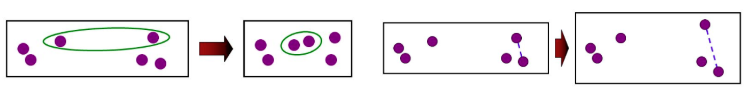
\includegraphics[width=7cm,height=5cm,keepaspectratio]{both.PNG}
\caption{\label{fig:1-Dress Work flow} Must Link and Cannot Link Constraints}
\end{figure}

Given a Dataset D Let $\zeta$ denote the set of discovered clusters in D. A ML constraint {x, y} is satisfied if both constrained objects are within the same cluster.
A NL constraint {x, y} is satisfied if both constrained objects are not within the same cluster, i.e.  holds true. Building on these two approaches, the goal of our method is as follows:\\

Given dataset D and a set of ML/NL constraints,find subspace S that best describes the concept, as reflected in the constraints, where ”best” refers to cluster quality and constraint satisfaction.\\

A Key assumption taken into account is that a subspace is of higher importance and is relevant regarding the target concept,if ML constrained objects have lower distance and its corresponding NL constraint 
Objects have higher distances to each other.This approach uses constraints to score and compare the quality rather than adjusting the clusters. This approach seeks subspaces seeking those clusters.\\

This approach uses no labels and smaller number of constraints to find subspaces.These constraints guide the creation of the subspaces.How this approach works is that DRESS looks for subspaces that contains well-
separated clusters which has satisfied all constraints. It then derives a score for each those subspaces. It considers high quality subspaces from those subspaces and by adding additional features to it expands the subspaces iteratively.In the expansion process the selection of high quality subspaces depends on the quality of the features getting added. If the feature getting added provides high quality clusters with all satisfied constraints then that subspace is selected for the further iterative process.\\

The work flow of DRESS can be best described using the following diagram which explains,

\begin{figure}[H]
\centering
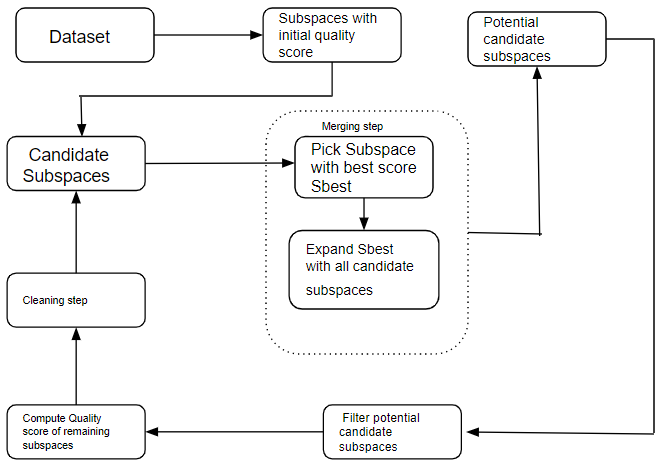
\includegraphics[width=20cm,height=5cm,keepaspectratio]{dress.PNG}
\caption{\label{fig:1-Dress Work flow} Dress Algorithm Work flow[1]}
\end{figure}

In figure \ref{fig:1-Dress Work flow} the approach generates potential candidate subspaces  and selects the current best subspace by assigning quality scores to each subspaces.The current best subspace is later merged with additional features,thus generating set of potential candidate subspaces and iteratively the process continues with the quality score calculation till we end up with one best subspace score containing all the best features in it.\\

The quality score is calculated by performing filtering operations on the candidate subspaces where we apply a different clustering approach which will be explained later in the clustering approach section below.

\subsection{Scoring of subspace in DRESS}
We have used the same quality score calculation which is done using a custom quality function which ranks the subspace using two criteria mentioned in the paper. It does so by evaluating the subspaces by 
(1)the degree to which constraints are satisfied and (2) the distance between constrained objects in the subspace.\cite{tommy}

(1) We assume that the subspace consists of dense regions of similar objects.The subspace consists of clusters where ML objects are within the same cluster and Nl objects are in different clusters.In the proposed
approach the found groups of similar objects are modeled as follows, If there exits a set of satisfied ML and NL constraints respectively for ML and NL constraints, the quality function is derived as\\
\begin{equation}
q_{cons} = \dfrac{|ML_{sat}(S)|+|NL_{sat}(S)|}{|ML|+|NL|}
\end{equation}

The above mentioned ranks the subspace on constraints satisfaction. But the author had two major problems with this approach,If the algorithm chooses more than one subspace with same constraints there may exist more than 
one subspace which will be termed important or best and the author also considered the distance between the ML pairs and NL pairs, where in the distance between the Nl pairs must be greater than ML pairs else there maybe 
considerable situations where NL objects maybe more similar than ML objects which contradicts the assumption made which in turn leads to subspace not representing the target concept. To avoid these two scenarios the author takes 
into account the average distances between the ML and NL pairs, where the distance function is defined as
\begin{equation}
q_{dist(S)} = {d^{NL}_{avg}(S)-d^{ML}_{avg}(S)}
%$X^{j}_L
\end{equation}

The distance function used in the above approach is HEOM Heterogeneous Euclidean
Overlap Metric (HEOM), that deals with both continuous and nominal features.
The quality function we obtain in the end with all our scenarios are this one
\begin{equation}
q_{(S)} = {q_{cons}(S)*q_{dist}(S)}
\end{equation}
%$d^{NL}_{avg}(S)=\sum_{{x,y}\in NL} \frac{d(S,x,y)}{|NL|} $
%$d^{ML}_{avg}(S)=\sum_{{x,y}\in NL} \frac{d(S,x,y)}{|NL|} $

\section{Clustering Approach}
\subsection{Filtering Subspaces}
We have implemented a different approach to the normal clustering process.This approach extends density based clustering algorithm such as DBSCAN in a semi-supervised way. At first we make use of both labeled and unlabeled data to determine the density-based parameters(Minpts and Eps).Once we have the information, local clusters are constructed by applying DBSCAN on the target dataset(different parameters set) and these local clusters are integrated to obtain the final results.\\

Firstly, we have assumed that each class of instances are constructed in different size,shape and density leading to an assumption that in density-based approaches different set of parameters can result in different clustering results.
Henceforth it is necessary to define individual set of parameters for each cluster.

Given a labeled and unlabeled set, a subset constituting a labeled set with class label j and unlabeled set is constructed. A random labeled data point x1 as shown in figure \ref{fig:3-Clustering 1} is selected as our seed point from the labeled set and its  closest neighbor is found. The distance between the closest point from our seed point is calculated using r =min \{dist($X_{1}$,$X_{2}$) $\mid X_{1} \in X^{j}_L,X_{2} \in X^{j}_L$ \}.

\begin{figure}[H]
\centering
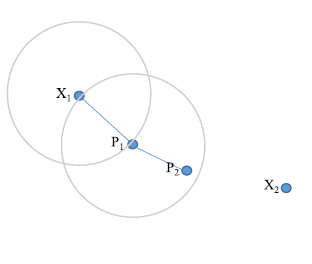
\includegraphics[width=20cm,height=5cm,keepaspectratio]{myraimage.png}
\caption{\label{fig:3-Clustering 1} Clustering process}
\end{figure}
These both data points are formed  as a new subset D and removed from the subset. Next we randomly move our data point to another point in the space say p2 as in figure \ref{fig:4-Clustering 1} and check its distance. If the distance between the randomly selected candidate point p2 and  any point in the subset is not greater than the radius r, then we move the candidate point in to our new subset D. This process is iteratively repeated until we achieve convergence(Till no data points are moved).
\begin{figure}[H]
\centering
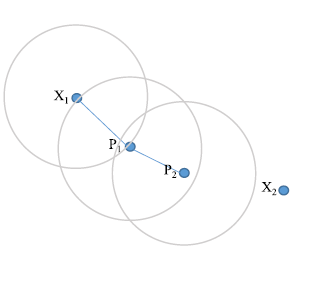
\includegraphics[width=20cm,height=5cm,keepaspectratio]{23.png}
\caption{\label{fig:4-Clustering 1} Clustering process}
\end{figure}

Now we check the newly created subset D whether it contains entire labeled set. If true we set the radius Eps value to the r for that labeled set J, otherwise we increase the length of the radius as in figure \ref{fig:5-Clustering 1} and keep on iterating this step until all the labeled dataset are in the same cluster\cite{adapt}.After Eps values are obtained we set the minpts. 
\begin{figure}[H]
\centering
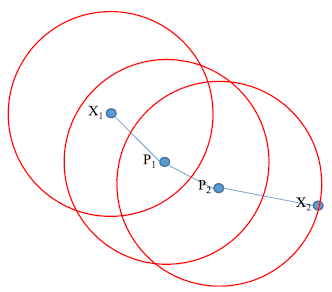
\includegraphics[width=20cm,height=5cm,keepaspectratio]{weq.png}
\caption{\label{fig:5-Clustering 1} Clustering process}
\end{figure}

Here in our approach we are changing the algorithm slightly in a way which suits our large dataset. We set the minpts value in a different way. Instead of assigning the minpts value directly we add the first instance and the last instance of the dataset and divide the value by 2. This is our new minpts value. After we have our minpts value we apply DBSCAN on the subset consisted of labeled set and unlabeled set with pair of parameters.After the clustering results are obtained we examine whether the entire labeled set is grouped into one cluster.This increased our processing time from O(n) to O(log n)

%If so we update the parameters and run DBSCAN on the updated parameters the algorithm runs till a labeled set is no longer grouped into one cluster.The process can be explained in the algorithm given below.

\subsection{Algorithm}

\begin{algorithm}
\caption{Density-Approach}
\hspace*{\algorithmicindent} \textbf{\small Input:X=$X_{L} \cup X_{U}$, labeled set $X_{L}$ and unlabeled set $X_{U}$} \\
\hspace*{\algorithmicindent} \textbf{Output:Class label on X}
\begin{algorithmic}[1]
\For{\texttt{each class j}}
\State {\small $X^{'}$=$X^{j}_L \cup X_{U}$ labeled set X j with class label j , set D = Ø;}
\State{\footnotesize Randomly select a labeled data point $X_{1}$ as initial seed point $X_{1} \in X^{j}_L$}
\State{Find its closest neighbor}
\State{\small $X_{2} \in X^{'}$,r =min \{dist($X_{1}$,$X_{2}$) $\mid X_{1} \in X^{j}_L,X_{2} \in X^{j}_L$ \}}
\While{}
\While{D doesn't change}
\State set D=[$X_{1}$,$X_{2}$],$X^{'}$= $X^{'}$-D
\State \textbf{If}(dist(x,p) $\leqq$ r$\mid$ x $\in$ X ,p $\in$ D) 
\State Update the subsets D = D+X and $X^{'}=X^{'}-D$
\State end \textbf{If}
\EndWhile
\State \textbf{end While}
\State \textbf{If} {\footnotesize subset D contains entire labeled set $X^{j}_L, D \cap X^{j}_L = X^{j}_L$}
\State $Eps_{j}=r$;Break
\State else r=r+0.1r
\State end \textbf{If}
\EndWhile
\State \textbf{end While}
\State Set MinPts = $(NoOfInstances/2)$
\While{}
\State Get clustering result $P_{j}$
\State {\small $by applying DBSCAN(Eps_{j},MinPts) on X^{j}_L \cup X_U $}
\State \textbf{If}{\small all points of $X^{j}_L$ are not in the same cluster of $P_{j}$}
\State LastInstance = $MinPts_{j}$
\State FirstInstance = FirstInstance
\State {\small $MinPts_{j}$ = (FirstInstance + LastInstance) / 2;Break}
\State \textbf{else}:
\State FirstInstance = $MinPts_{j}$              
\State LastInstance = LastInstance
\State {\small $MinPts_{j}$ = (FirstInstance + LastInstance) / 2;Break}
%$MinPts_{j}=MinPts+1$
\State end \textbf{If}
\EndWhile
\State \textbf{end While}
\State $density_{j}=MinPts_{j}/Eps_{j}$
\EndFor
\State end \textbf{for}
\State sort the class density {$density_{j}$}in a descending order:
\State \{$density^{s}_j \mid density^{m}_j  density^{m+1}_j $\}
\For{\textbf{s}}
\State Find the corresponding clustering result $P_{j}$ for the class density $density^{s}_j$
\State \textbf{If} {\small $X^{j}_U \subseteq X_U$ and $X^{j}_L$ is grouped in the same cluster by $P_{j}$}
\State Assign class label j to unlabeled set $X^{j}_U$
\State end \textbf{If}
\EndFor
\State end \textbf{for}
\State set x $\in X_U$ with any label as noise
\end{algorithmic}
\end{algorithm}

\subsection{Integration of local clusters}
After having got both of Eps and minpts values for all the classes, density is calculated using ${density_j = MinPts_j / Eps_j}$, and local clusters $p_j$.Then we sort the density values and look though with the highest one.If a set of unlabeled point is grouped with a labeled point then we group those unlabeled point with the labeled point by assigning the same class label. For example, if a set of unlabeled points are grouped with a labeled point with class label A then we assign class label A to those set of unlabeled points, This comes from the initial assumption that the points which lie in the same cluster should be of the same class.The process iterates over the set of density values. If at the end there exist a unlabeled point not belonging to or grouped to any labeled point then this unlabeled point is considered as noise.But if there is an overlap between two clusters we tend to consider the part of the cluster which has high density and assign the unlabeled point to that cluster.



\section{Evaluation Result}
For our evaluation we have considered two classifier to evaluate our model. These two classifiers have an advantage, the main being they can be used both as a classification and also a regression problem.One classifier being Random Forest can help us greatly in identifying relative importance of each feature on the prediction,second being Support Vector machine(SVM) which can also help us achieve our tasks.Using these classifiers We also add various other parameters on which we evaluate our data.
Our evaluation consists of these three phases
\begin{itemize}
\item We perform training and testing on various 
random seed points.
\item There has been a fixed number of constraints and 
its corresponding labels set.
\item Model runs on various seed points and we record
accuracy 
\end{itemize}

\subsection{Evaluation 1}
We have taken two class labels of 60 each and we set the no of constraints to 50.
we run our model on various seed points based off of these measures.\\
Parameters:
\begin{itemize}
\item $Label[0]$ = 25
\item $Label[1]$ = 75
\item Noofconstraints = 100
\end{itemize}

\begin{figure}[H]
\centering
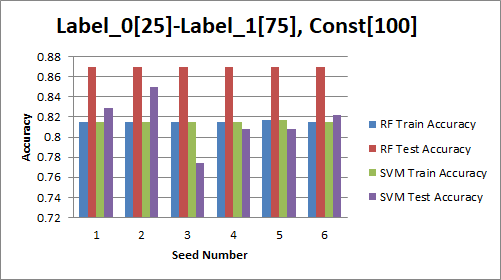
\includegraphics[width=7cm,height=5cm,keepaspectratio]{1.png}
\caption{\label{fig:2-Evaluation 1} Evaluation 1}
\end{figure}

We can see the accuracy for these parameters from the table.



\subsection{Evaluation 2}
We have taken two class labels of 60 each and we set the no of constraints to 50.
we run our model on various seed points based off of these measures.\\
Parameters:
\begin{itemize}
\item $Label[0]$ = 25
\item $Label[1]$ = 75
\item Noofconstraints = 50
\end{itemize}

\begin{figure}[H]
\centering
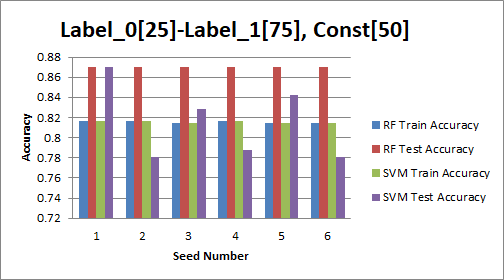
\includegraphics[width=7cm,height=5cm,keepaspectratio]{2.png}
\caption{\label{fig:2-Evaluation 2} Evaluation 2}
\end{figure}

We can see the accuracy for these parameters from the table.

\subsection{Evaluation 3}
We have taken two class labels of 60 each and we set the no of constraints to 50.
we run our model on various seed points based off of these measures.\\
Parameters:
\begin{itemize}
\item $Label[0]$ = 60
\item $Label[1]$ = 60
\item Noofconstraints = 100
\end{itemize}

\begin{figure}[H]
\centering
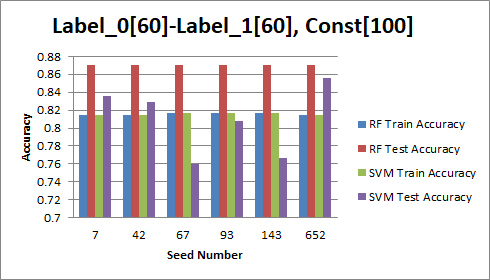
\includegraphics[width=7cm,height=5cm,keepaspectratio]{3.png}
\caption{\label{fig:2-Evaluation 3} Evaluation 3}
\end{figure}

We can see the accuracy for these parameters from the table.


\subsection{Evaluation 4}
We have taken two class labels of 60 each and we set the no of constraints to 50.
we run our model on various seed points based off of these measures.\\
Parameters:
\begin{itemize}
\item $Label[0]$ = 60
\item $Label[1]$ = 60
\item Noofconstraints = 50
\end{itemize}

\begin{figure}[H]
\centering
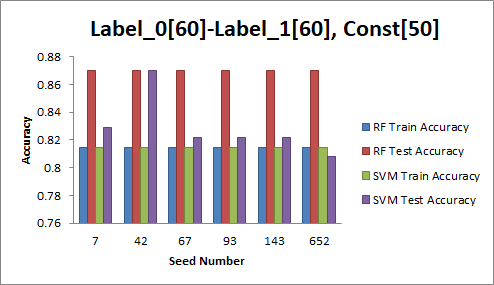
\includegraphics[width=7cm,height=5cm,keepaspectratio]{4.png}
\caption{\label{fig:2-Evaluation 4} Evaluation 4}
\end{figure}

We can see the accuracy for these parameters from the table

\subsection{Evaluation Summary}
We show all of the acquired results with all of the seed points.
\begin{figure}[H]
\centering
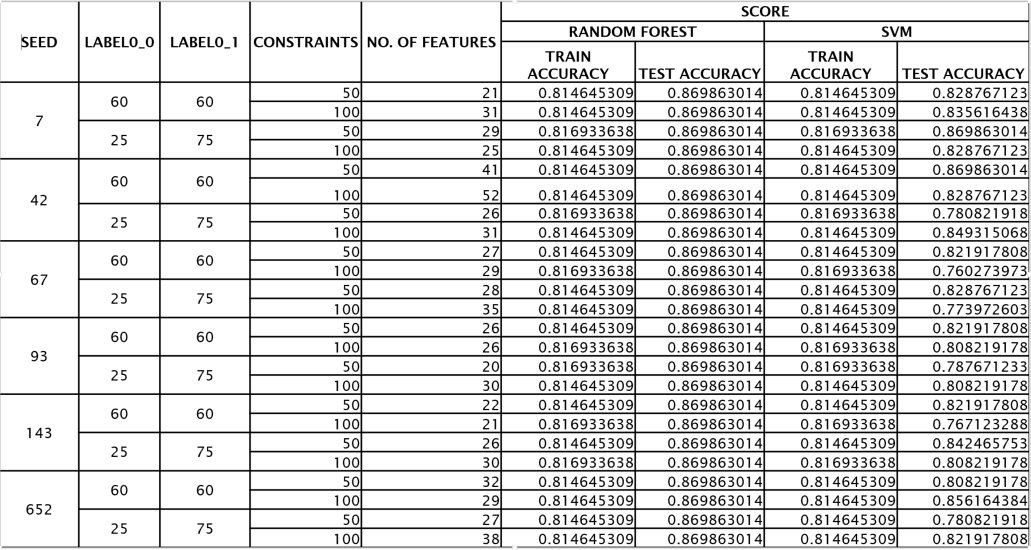
\includegraphics[width=8cm,height=7cm]{eval.PNG}
\caption{\label{fig:2-Evaluation 4} Evaluation 4}
\end{figure}

% \begin{tabular}{ |p{1cm}|p{1cm}|p{1.5cm}|p{1.5cm}|p{1.5cm}|  }
% \hline
% \multicolumn{5}{|c|}{Evaluation 4} \\
% \hline
% Country Name     or Area Name& ISO ALPHA 2 Code &ISO ALPHA 3&ISO ALPHA 3&ISO ALPHA 3 \\
% \hline
% Afghanistan & AF &AFG \\
% Aland Islands & AX   & ALA \\
% Albania &AL & ALB \\
% Algeria    &DZ & DZA \\
% American Samoa & AS & ASM \\
% Andorra & AD & AND   \\
% Angola & AO & AGO \\
% \hline
% \end{tabular}\\



\section{Challenges Faced in Implementation}
We faced few challenges which we dealt with while implementing our approach
few will be listed below
\begin{itemize}
\item Distance Calculation
 \subitem 1.Vectorized implementation for distance
 \subitem 2.Calculated on basis of categorical and numerical 
we reduced so many for loops of distance 
calculation by using numpy array functionalities

\item MinPoints
\subitem incorporated a binary search approach\\
(Using binary search approach we reduced running time from 5 days to 2.5 days)

\item Parallel Programming\\
We implemented parallel programming which 
\subitem Used all cores of system for efficient processing
\subitem Memory error(solved by reducing cores)\\
(Using this we reduced running time from 2.5 days to 3
-5 hours. Used 16 cores of the system.)
\end{itemize}

\section{Conclusion \& Future work}
We conclude here by saying Our incorporated approach gave more features when compared 
with DRESS Algorithm.We managed to improve the accuracy by 2\% when compared to DRESS.
Results from SVM Classifier was better when compared with DRESS rather than the results from random forest classifier.
Random forest Classifier gave same accuracy when compared with DRESS since RF takes best of all combinations.

For future work, different clustering approaches can be incorporated to extend the accuracy further.
The literature survey also provided us with different Dimension selection and Dimension 
weighting approaches[3] which could be incorporated to further improve the algorithm. 
  
\bibliographystyle{plain}
\bibliography{bibliography.bib}


\end{document}
